\chapter{Sleep}
Flash an XBee with the End-Device AT firmware using X-CTU.
First, plug the XBee in the XBee explorer socket and connect the USB cable.
Use the \texttt{dmesg} command to find to which device is the USB attached.
Look for a line similar to

\texttt{[ 6370.421000] usb 3-2.2: FTDI USB Serial Device converter now attached to ttyUSB0}

The command to invoke X-CTU will be something similar to

\texttt{wine .wine/drive\_c/Program{\textbackslash} Files/Digi/XCTU/X-CTU.exe}

Then set the port as in Fig. \ref{fig:set-port} and test that you can connect to the XBee using the ``Test/Query'' button as in Fig.~\ref{fig:test-xtu}.
\begin{figure}[htbp]
  \centering
  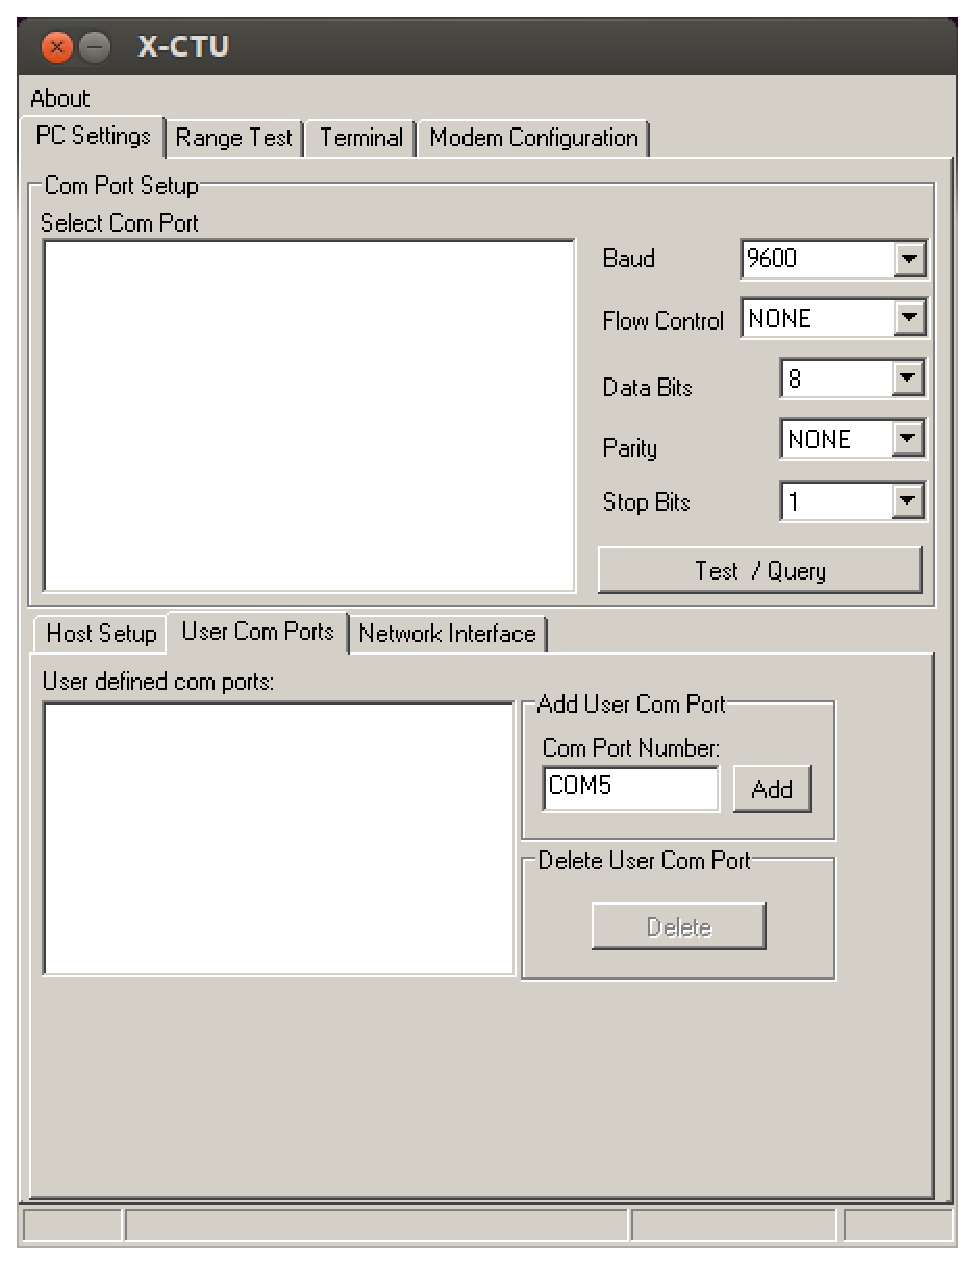
\includegraphics[width=0.3\linewidth]{figures/set-port.eps}
  \caption{LDR}
  \label{fig:set-port}
\end{figure}

\begin{figure}[htbp]
  \centering
  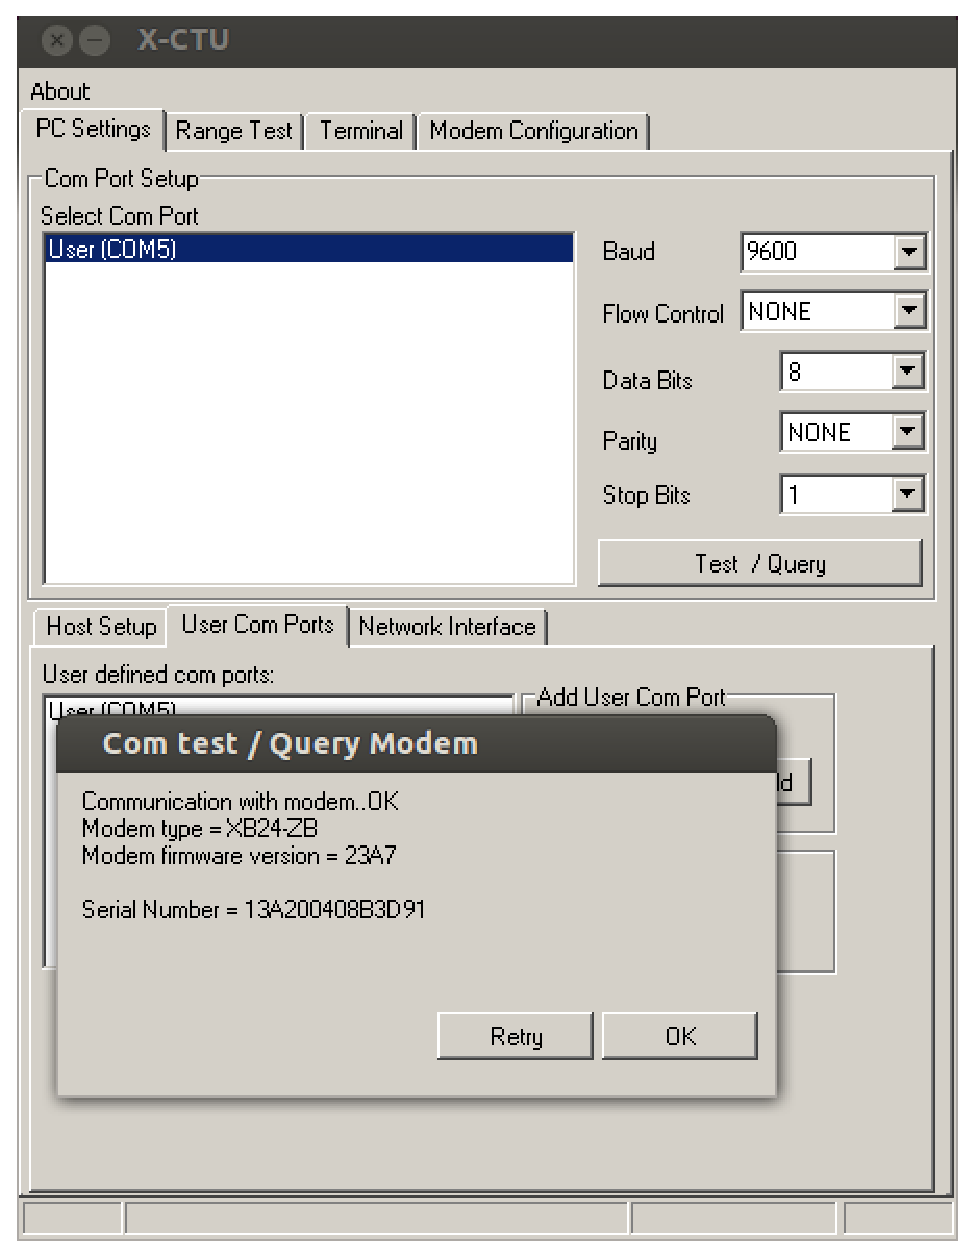
\includegraphics[width=0.3\linewidth]{figures/test-xctu.eps}
  \caption{LDR}
  \label{fig:test-xctu}
\end{figure}
